% Options for packages loaded elsewhere
\PassOptionsToPackage{unicode}{hyperref}
\PassOptionsToPackage{hyphens}{url}
%
\documentclass[
]{article}
\usepackage{amsmath,amssymb}
\usepackage{iftex}
\ifPDFTeX
  \usepackage[T1]{fontenc}
  \usepackage[utf8]{inputenc}
  \usepackage{textcomp} % provide euro and other symbols
\else % if luatex or xetex
  \usepackage{unicode-math} % this also loads fontspec
  \defaultfontfeatures{Scale=MatchLowercase}
  \defaultfontfeatures[\rmfamily]{Ligatures=TeX,Scale=1}
\fi
\usepackage{lmodern}
\ifPDFTeX\else
  % xetex/luatex font selection
\fi
% Use upquote if available, for straight quotes in verbatim environments
\IfFileExists{upquote.sty}{\usepackage{upquote}}{}
\IfFileExists{microtype.sty}{% use microtype if available
  \usepackage[]{microtype}
  \UseMicrotypeSet[protrusion]{basicmath} % disable protrusion for tt fonts
}{}
\makeatletter
\@ifundefined{KOMAClassName}{% if non-KOMA class
  \IfFileExists{parskip.sty}{%
    \usepackage{parskip}
  }{% else
    \setlength{\parindent}{0pt}
    \setlength{\parskip}{6pt plus 2pt minus 1pt}}
}{% if KOMA class
  \KOMAoptions{parskip=half}}
\makeatother
\usepackage{xcolor}
\usepackage[margin=1in]{geometry}
\usepackage{longtable,booktabs,array}
\usepackage{calc} % for calculating minipage widths
% Correct order of tables after \paragraph or \subparagraph
\usepackage{etoolbox}
\makeatletter
\patchcmd\longtable{\par}{\if@noskipsec\mbox{}\fi\par}{}{}
\makeatother
% Allow footnotes in longtable head/foot
\IfFileExists{footnotehyper.sty}{\usepackage{footnotehyper}}{\usepackage{footnote}}
\makesavenoteenv{longtable}
\usepackage{graphicx}
\makeatletter
\def\maxwidth{\ifdim\Gin@nat@width>\linewidth\linewidth\else\Gin@nat@width\fi}
\def\maxheight{\ifdim\Gin@nat@height>\textheight\textheight\else\Gin@nat@height\fi}
\makeatother
% Scale images if necessary, so that they will not overflow the page
% margins by default, and it is still possible to overwrite the defaults
% using explicit options in \includegraphics[width, height, ...]{}
\setkeys{Gin}{width=\maxwidth,height=\maxheight,keepaspectratio}
% Set default figure placement to htbp
\makeatletter
\def\fps@figure{htbp}
\makeatother
\setlength{\emergencystretch}{3em} % prevent overfull lines
\providecommand{\tightlist}{%
  \setlength{\itemsep}{0pt}\setlength{\parskip}{0pt}}
\setcounter{secnumdepth}{5}
\usepackage{booktabs}
\ifLuaTeX
  \usepackage{selnolig}  % disable illegal ligatures
\fi
\usepackage[]{natbib}
\bibliographystyle{apalike}
\IfFileExists{bookmark.sty}{\usepackage{bookmark}}{\usepackage{hyperref}}
\IfFileExists{xurl.sty}{\usepackage{xurl}}{} % add URL line breaks if available
\urlstyle{same}
\hypersetup{
  pdftitle={Homeworks for James' Stats classes},
  pdfauthor={Zhifei Yu},
  hidelinks,
  pdfcreator={LaTeX via pandoc}}

\title{Homeworks for James' Stats classes}
\author{Zhifei Yu}
\date{2023-7-14}

\begin{document}
\maketitle

{
\setcounter{tocdepth}{2}
\tableofcontents
}
\hypertarget{welcome}{%
\section*{Welcome!}\label{welcome}}
\addcontentsline{toc}{section}{Welcome!}

Howdy! This is a collection of 4 assignments from James Scott's probability and Statistics courses, written by Zhifei Yu a.k.a Kevin.

\hypertarget{homework-1}{%
\section{Homework 1}\label{homework-1}}

\hypertarget{problem-1-playlists-revisited}{%
\subsection{Problem 1 Playlists revisited}\label{problem-1-playlists-revisited}}

\hypertarget{part-a}{%
\subsubsection{Part A}\label{part-a}}

\begin{longtable}[]{@{}
  >{\centering\arraybackslash}p{(\columnwidth - 4\tabcolsep) * \real{0.1250}}
  >{\centering\arraybackslash}p{(\columnwidth - 4\tabcolsep) * \real{0.1111}}
  >{\centering\arraybackslash}p{(\columnwidth - 4\tabcolsep) * \real{0.1111}}@{}}
\toprule\noalign{}
\begin{minipage}[b]{\linewidth}\centering
~
\end{minipage} & \begin{minipage}[b]{\linewidth}\centering
0
\end{minipage} & \begin{minipage}[b]{\linewidth}\centering
1
\end{minipage} \\
\midrule\noalign{}
\endhead
\bottomrule\noalign{}
\endlastfoot
\textbf{0} & 0.925 & 0.912 \\
\textbf{1} & 0.075 & 0.088 \\
\end{longtable}

Column:

0: never plays Daft Punk

1: plays Daft Punk

Row:

0: never plays David Bowie

1: plays David Bowie

\hypertarget{part-b}{%
\subsubsection{Part B}\label{part-b}}

To check out if 2 events are independent, we can use the definition: If A and B are independent, then P(A\textbar B) = P(A\textbar\textasciitilde B) = P(A) To make it clear, ``plays Pink Floyd'' is considered as event B, ``plays Johnny cash'' is event A.

\begin{longtable}[]{@{}
  >{\centering\arraybackslash}p{(\columnwidth - 2\tabcolsep) * \real{0.0972}}
  >{\centering\arraybackslash}p{(\columnwidth - 2\tabcolsep) * \real{0.0972}}@{}}
\toprule\noalign{}
\begin{minipage}[b]{\linewidth}\centering
0
\end{minipage} & \begin{minipage}[b]{\linewidth}\centering
1
\end{minipage} \\
\midrule\noalign{}
\endhead
\bottomrule\noalign{}
\endlastfoot
0.94 & 0.06 \\
\end{longtable}

0: never plays Johnny Cash

1: plays Johnny Cash

\begin{longtable}[]{@{}
  >{\centering\arraybackslash}p{(\columnwidth - 4\tabcolsep) * \real{0.1250}}
  >{\centering\arraybackslash}p{(\columnwidth - 4\tabcolsep) * \real{0.1111}}
  >{\centering\arraybackslash}p{(\columnwidth - 4\tabcolsep) * \real{0.1111}}@{}}
\toprule\noalign{}
\begin{minipage}[b]{\linewidth}\centering
~
\end{minipage} & \begin{minipage}[b]{\linewidth}\centering
0
\end{minipage} & \begin{minipage}[b]{\linewidth}\centering
1
\end{minipage} \\
\midrule\noalign{}
\endhead
\bottomrule\noalign{}
\endlastfoot
\textbf{0} & 0.945 & 0.895 \\
\textbf{1} & 0.055 & 0.105 \\
\end{longtable}

Column:

0: never plays Johnny Cash

1: plays Johnny Cash

Row:

0: never plays Pink Floyd

1: plays Pink Floyd

So, in this case P(A) = 6\%, P(A\textbar B) = 10.5\%, P(A\textbar not B) = 5.5\%; clearly, they are not equal. Therefore, they are not independent and seem to have positive relationship.

Or we can check it by if P(B) = P(B\textbar A) = P(B\textbar\textasciitilde A)

\begin{longtable}[]{@{}
  >{\centering\arraybackslash}p{(\columnwidth - 2\tabcolsep) * \real{0.1111}}
  >{\centering\arraybackslash}p{(\columnwidth - 2\tabcolsep) * \real{0.1111}}@{}}
\toprule\noalign{}
\begin{minipage}[b]{\linewidth}\centering
0
\end{minipage} & \begin{minipage}[b]{\linewidth}\centering
1
\end{minipage} \\
\midrule\noalign{}
\endhead
\bottomrule\noalign{}
\endlastfoot
0.895 & 0.105 \\
\end{longtable}

0: never plays Pink Floyd

1: plays Pink Floyd

\begin{longtable}[]{@{}
  >{\centering\arraybackslash}p{(\columnwidth - 4\tabcolsep) * \real{0.1250}}
  >{\centering\arraybackslash}p{(\columnwidth - 4\tabcolsep) * \real{0.0833}}
  >{\centering\arraybackslash}p{(\columnwidth - 4\tabcolsep) * \real{0.1111}}@{}}
\toprule\noalign{}
\begin{minipage}[b]{\linewidth}\centering
~
\end{minipage} & \begin{minipage}[b]{\linewidth}\centering
0
\end{minipage} & \begin{minipage}[b]{\linewidth}\centering
1
\end{minipage} \\
\midrule\noalign{}
\endhead
\bottomrule\noalign{}
\endlastfoot
\textbf{0} & 0.9 & 0.817 \\
\textbf{1} & 0.1 & 0.183 \\
\end{longtable}

Column:

0: never plays Pink Floyd

1: plays Pink Floyd

Row:

0: never plays Johnny Cash

1: plays Johnny Cash

Clearly, P(B) = 10.5\%, P(B\textbar A) = 18.3\%, and P(B\textbar\textasciitilde A) = 10\%, so they are not close to each other.

\hypertarget{problem-2-super-bowl-ads}{%
\subsection{Problem 2 Super Bowl ads}\label{problem-2-super-bowl-ads}}

\hypertarget{part-a-1}{%
\subsubsection{Part A}\label{part-a-1}}

\begin{longtable}[]{@{}
  >{\centering\arraybackslash}p{(\columnwidth - 2\tabcolsep) * \real{0.1111}}
  >{\centering\arraybackslash}p{(\columnwidth - 2\tabcolsep) * \real{0.1111}}@{}}
\toprule\noalign{}
\begin{minipage}[b]{\linewidth}\centering
FALSE
\end{minipage} & \begin{minipage}[b]{\linewidth}\centering
TRUE
\end{minipage} \\
\midrule\noalign{}
\endhead
\bottomrule\noalign{}
\endlastfoot
0.7 & 0.3 \\
\end{longtable}

True: should be danger

False: not danger

Which returns the results that P(danger = TRUE) = 30\%

\begin{longtable}[]{@{}
  >{\centering\arraybackslash}p{(\columnwidth - 4\tabcolsep) * \real{0.1667}}
  >{\centering\arraybackslash}p{(\columnwidth - 4\tabcolsep) * \real{0.1111}}
  >{\centering\arraybackslash}p{(\columnwidth - 4\tabcolsep) * \real{0.1111}}@{}}
\toprule\noalign{}
\begin{minipage}[b]{\linewidth}\centering
~
\end{minipage} & \begin{minipage}[b]{\linewidth}\centering
FALSE
\end{minipage} & \begin{minipage}[b]{\linewidth}\centering
TRUE
\end{minipage} \\
\midrule\noalign{}
\endhead
\bottomrule\noalign{}
\endlastfoot
\textbf{FALSE} & 0.88 & 0.61 \\
\textbf{TRUE} & 0.12 & 0.39 \\
\end{longtable}

Column:

True: should be danger

False: not danger

Row:

True: should be funny

False: not funny

From the table, we can know that:

P(danger = TRUE \textbar{} funny = TRUE) = 39\%

P(danger = TRUE \textbar{} funny = FALSE) = 12\%

Undoubtedly, from this statistics, humor and danger are absolutely not independent because P(danger) ≠ P(danger\textbar funny) ≠ P(danger\textbar not funny)

It seems that humor are indeed more or less a indication of danger for this ads, because under the condition that ads are funny, the probability of danger seems to be higher than unconditional probability and under the another condition that ads are not funny, the probability of it shows way much lower than unconditional probability.

\hypertarget{part-b-1}{%
\subsubsection{Part B}\label{part-b-1}}

\begin{longtable}[]{@{}
  >{\centering\arraybackslash}p{(\columnwidth - 2\tabcolsep) * \real{0.1111}}
  >{\centering\arraybackslash}p{(\columnwidth - 2\tabcolsep) * \real{0.1111}}@{}}
\toprule\noalign{}
\begin{minipage}[b]{\linewidth}\centering
FALSE
\end{minipage} & \begin{minipage}[b]{\linewidth}\centering
TRUE
\end{minipage} \\
\midrule\noalign{}
\endhead
\bottomrule\noalign{}
\endlastfoot
0.63 & 0.37 \\
\end{longtable}

True: with animals False: without animals

Which returns the results that P(animals = TRUE) = 37\%

\begin{longtable}[]{@{}
  >{\centering\arraybackslash}p{(\columnwidth - 4\tabcolsep) * \real{0.1667}}
  >{\centering\arraybackslash}p{(\columnwidth - 4\tabcolsep) * \real{0.1111}}
  >{\centering\arraybackslash}p{(\columnwidth - 4\tabcolsep) * \real{0.1111}}@{}}
\toprule\noalign{}
\begin{minipage}[b]{\linewidth}\centering
~
\end{minipage} & \begin{minipage}[b]{\linewidth}\centering
FALSE
\end{minipage} & \begin{minipage}[b]{\linewidth}\centering
TRUE
\end{minipage} \\
\midrule\noalign{}
\endhead
\bottomrule\noalign{}
\endlastfoot
\textbf{FALSE} & 0.63 & 0.62 \\
\textbf{TRUE} & 0.37 & 0.38 \\
\end{longtable}

Column:

True: with animals

False: without animals

Row:

True: has sex contents

False: not have sex contents

From the table, we can know that:

P(animals = TRUE \textbar{} use\_sex = TRUE) = 38\%

P(animals = TRUE \textbar{} use\_sex = FALSE) = 37\%

From the probability tables and unconditional probability, I think animals and use\_sex are statistically independent.My argument is that the unconditional probability of animals seems to be very close to the conditional probabilities on both conditions that using sex and not using, which, from definition, shows this 2 events are independent.

\hypertarget{part-c}{%
\subsubsection{Part C}\label{part-c}}

\begin{longtable}[]{@{}
  >{\centering\arraybackslash}p{(\columnwidth - 2\tabcolsep) * \real{0.1111}}
  >{\centering\arraybackslash}p{(\columnwidth - 2\tabcolsep) * \real{0.1111}}@{}}
\toprule\noalign{}
\begin{minipage}[b]{\linewidth}\centering
FALSE
\end{minipage} & \begin{minipage}[b]{\linewidth}\centering
TRUE
\end{minipage} \\
\midrule\noalign{}
\endhead
\bottomrule\noalign{}
\endlastfoot
0.71 & 0.29 \\
\end{longtable}

True: with celebrities

False: without celebrities

Which returns the results that P(celebrity = TRUE) = 29\%

\begin{longtable}[]{@{}
  >{\centering\arraybackslash}p{(\columnwidth - 4\tabcolsep) * \real{0.1667}}
  >{\centering\arraybackslash}p{(\columnwidth - 4\tabcolsep) * \real{0.1111}}
  >{\centering\arraybackslash}p{(\columnwidth - 4\tabcolsep) * \real{0.1111}}@{}}
\toprule\noalign{}
\begin{minipage}[b]{\linewidth}\centering
~
\end{minipage} & \begin{minipage}[b]{\linewidth}\centering
FALSE
\end{minipage} & \begin{minipage}[b]{\linewidth}\centering
TRUE
\end{minipage} \\
\midrule\noalign{}
\endhead
\bottomrule\noalign{}
\endlastfoot
\textbf{FALSE} & 0.71 & 0.71 \\
\textbf{TRUE} & 0.29 & 0.29 \\
\end{longtable}

Column:

True: with celebrities

False: without celebrities

Row:

True: has patriotic contents

False: not have patriotic contents

From the table, we can know that:

P(celebrity = TRUE \textbar{} patriotic = TRUE) = 29\%

P(celebrity = TRUE \textbar{} patriotic = FALSE) = 29\%

Similar with Part B, in this part, the unconditional probability of celebrity is nearly equal to the 2 conditional probabilities of both showing patriotic contents and not showing this. Thus, they are independent on the basis of this data.

\hypertarget{problem-3-beauty-or-not-in-the-classroom}{%
\subsection{Problem 3 Beauty, or not, in the classroom}\label{problem-3-beauty-or-not-in-the-classroom}}

\hypertarget{part-a-2}{%
\subsubsection{Part A}\label{part-a-2}}

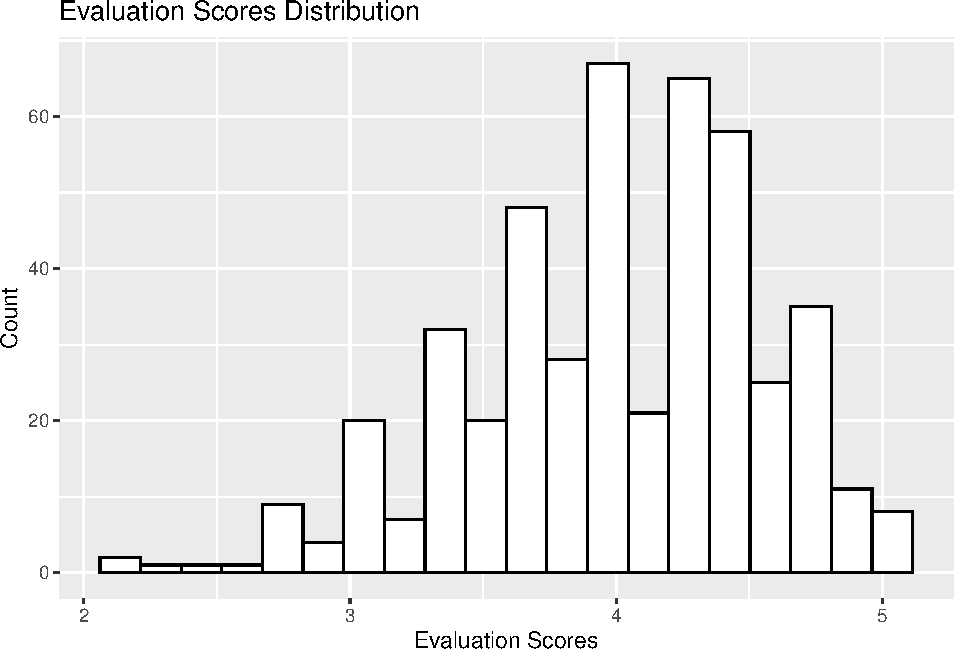
\includegraphics{_main_files/figure-latex/unnamed-chunk-17-1.pdf}

Above is the histogram plot that shows course evaluation scores of all professors.

X axis shows the evaluation scores which professors have gained.

Y axis shows tha counting of each score.

We can see around 4 is where the most scores are sited. So I guess that most UT's professor are pretty good so that they can get good evaluations scores from students.

\hypertarget{part-b-2}{%
\subsubsection{Part B}\label{part-b-2}}

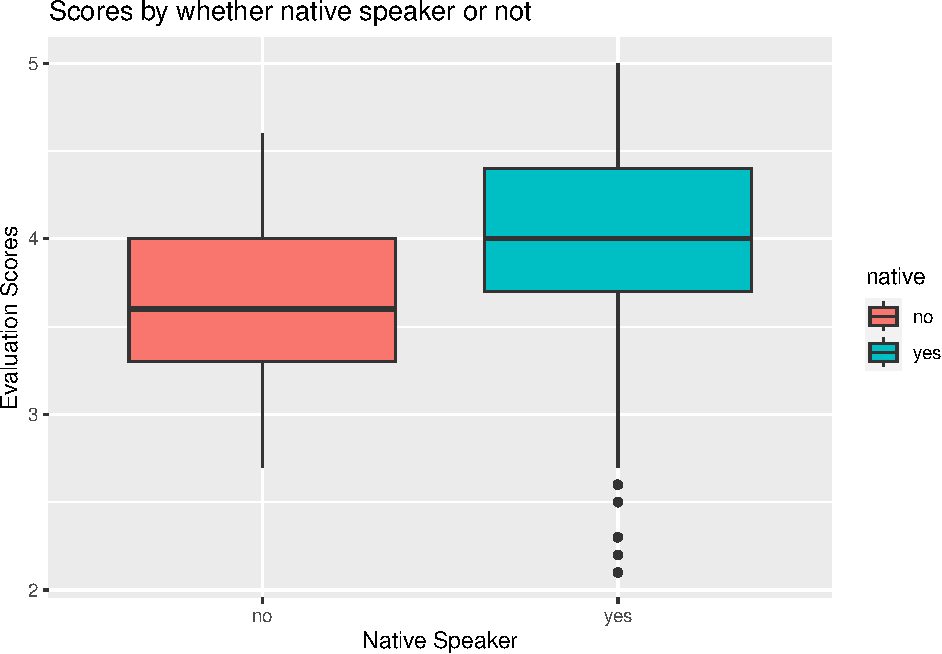
\includegraphics{_main_files/figure-latex/unnamed-chunk-18-1.pdf}

The left red box represents the non-native English speaker.

The right blue box stands for native speaker. Y axis means the evaluation scores.

So, from this boxplot, we can conclude that native speakers generally get better score than non-native speaker.

\hypertarget{part-c-1}{%
\subsubsection{Part C}\label{part-c-1}}

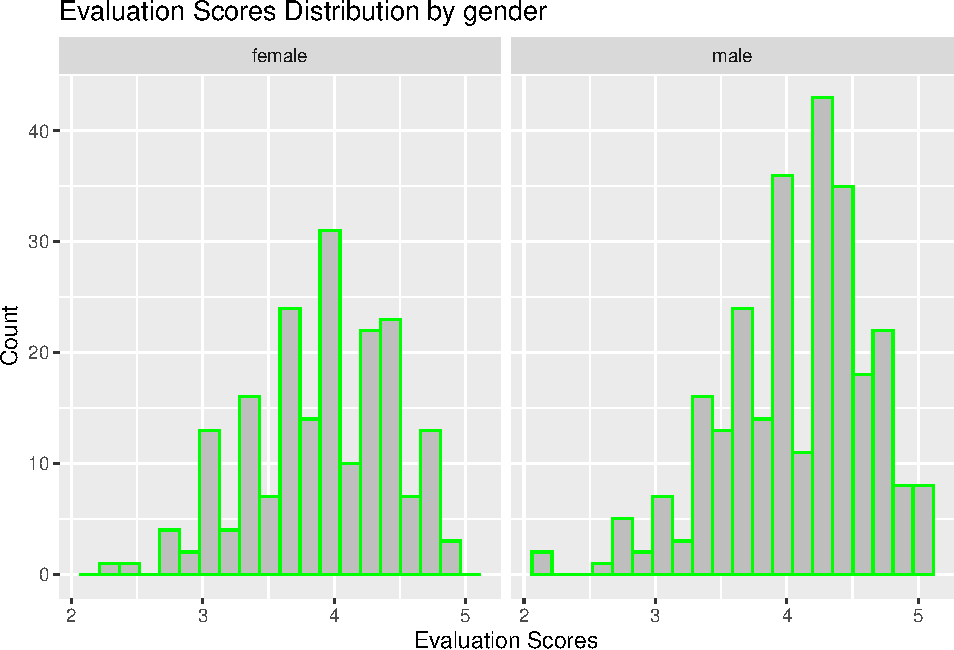
\includegraphics{_main_files/figure-latex/unnamed-chunk-19-1.pdf}

From this plot, we can see that male professors are more focused around 4, whereas female professors are more spread-out.

\hypertarget{part-d}{%
\subsubsection{Part D}\label{part-d}}

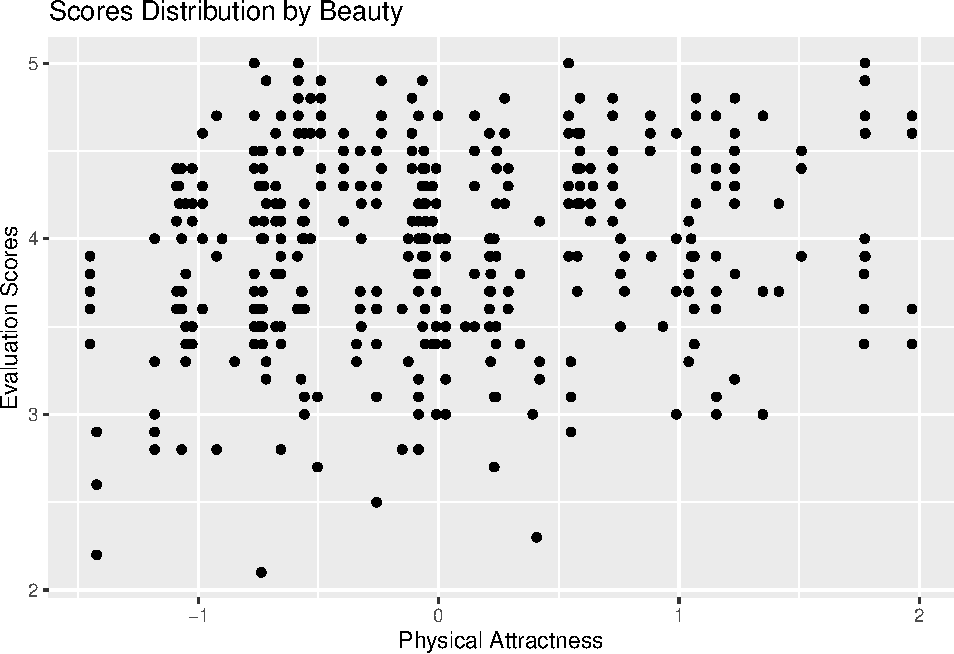
\includegraphics{_main_files/figure-latex/unnamed-chunk-20-1.pdf}

X axis stands for the score of beauty.

I think that the physical attraction basically has slightly positive relationship with evaluation scores but cannot be a predictive indicator of evaluation.

\hypertarget{problem-4-sat-scores-for-ut-students}{%
\subsection{Problem 4 SAT scores for UT students}\label{problem-4-sat-scores-for-ut-students}}

Scores

Mean

Std

IQR

quan5

quan25

median

quan75

quan95

1

SAT-V

595.05

83.77

110.00

460.00

540.00

590.00

650.00

730.00

2

SAT-Q

619.98

83.08

120.00

480.00

560.00

620.00

680.00

760.00

3

GPA

3.21

0.48

0.72

2.36

2.87

3.25

3.59

3.92

SAT-V means SAT verbal scores and SAT-Q means SAT quantitative score, while GPA means accumulative grade points.

Mean is the average of each score, std means standard deviation, IOR is inter-quantile range.

Quan5 is 5th percentile and so on so forth.

\hypertarget{problem-5-bike-sharing}{%
\subsection{Problem 5 bike sharing}\label{problem-5-bike-sharing}}

\hypertarget{plot-a}{%
\subsubsection{Plot A}\label{plot-a}}

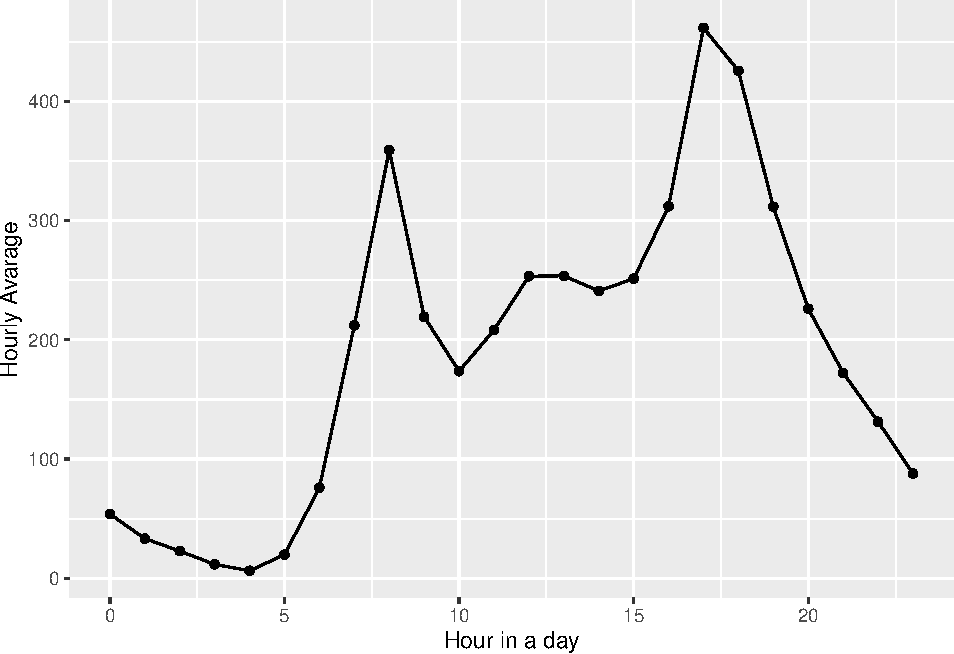
\includegraphics{_main_files/figure-latex/unnamed-chunk-23-1.pdf}

In this plot, x axis stands for the 24 hours in a single day. 0 is midnight and 10 is 10a.m., so on so forth.

Y is the average ridership of each hour throughout all days in this data.

We can see that the average ridership around morning rush hour and afternoon rush hour are 2 peaks. Also, it remains fairly high during daytime but swiftly decreases in the evening.

\hypertarget{plot-b}{%
\subsubsection{Plot B}\label{plot-b}}

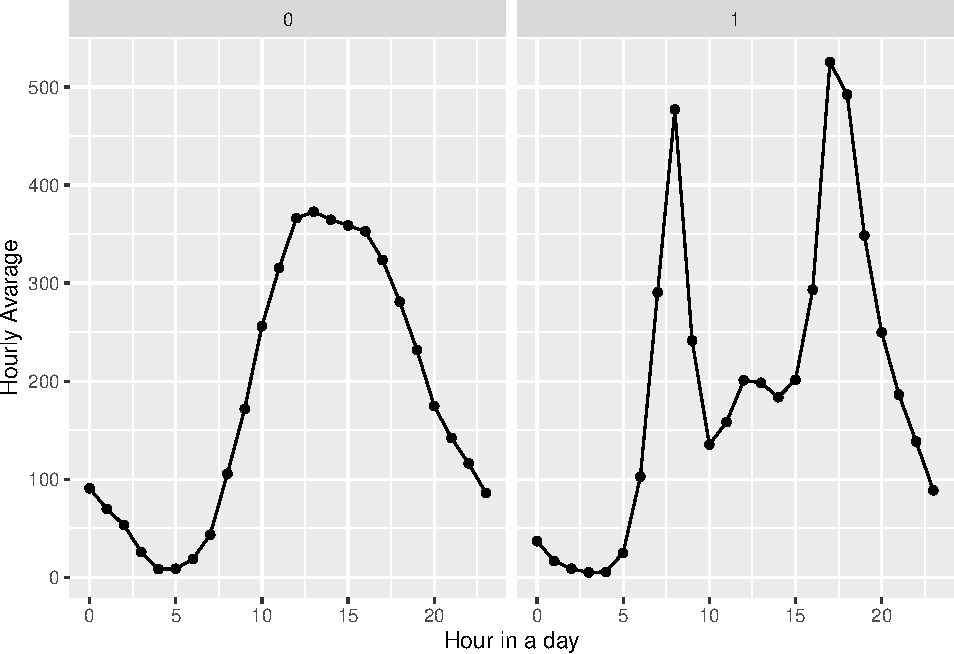
\includegraphics{_main_files/figure-latex/unnamed-chunk-24-1.pdf}

X and Y axis basically are the same as the plot A.

0 means weekends and holidays, while 1 means workdays. Workdays' pattern is pretty close to plot A and it complies with common sense. But non-holidays' pattern are quite different from Plot days, people tends to use bikes around noon till afternoon. I guess that people are likely to hang out during this time.

\hypertarget{plot-c}{%
\subsubsection{Plot C}\label{plot-c}}

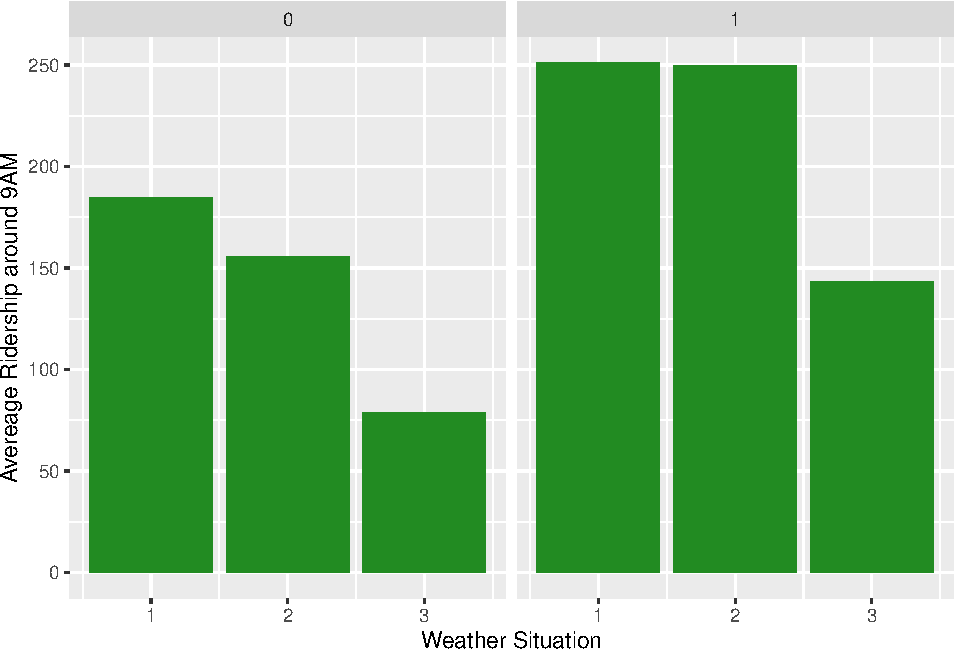
\includegraphics{_main_files/figure-latex/unnamed-chunk-25-1.pdf}

0 and 1 has the same meaning as Part B.

X axis means weather situation where 1 means sunny day, 2 means cloudy and misty day, and 3 means light snowy and light rainy day.

Y axis represents the avarage ridership around 9a.m.

So, in non-workdays, when the weather becomes cloudy, a few people may not go out riding bike because they might think that there will be potential rains. However, in workdays, almost all people will not change their original plan, which is getting a bike, just because of potential rains. They have to work!

\hypertarget{homework-2}{%
\section{Homework 2}\label{homework-2}}

\hypertarget{problem-1-capital-metro-ut-ridership}{%
\subsection{Problem 1 Capital Metro UT Ridership}\label{problem-1-capital-metro-ut-ridership}}

\hypertarget{plot-1}{%
\subsubsection{Plot 1}\label{plot-1}}

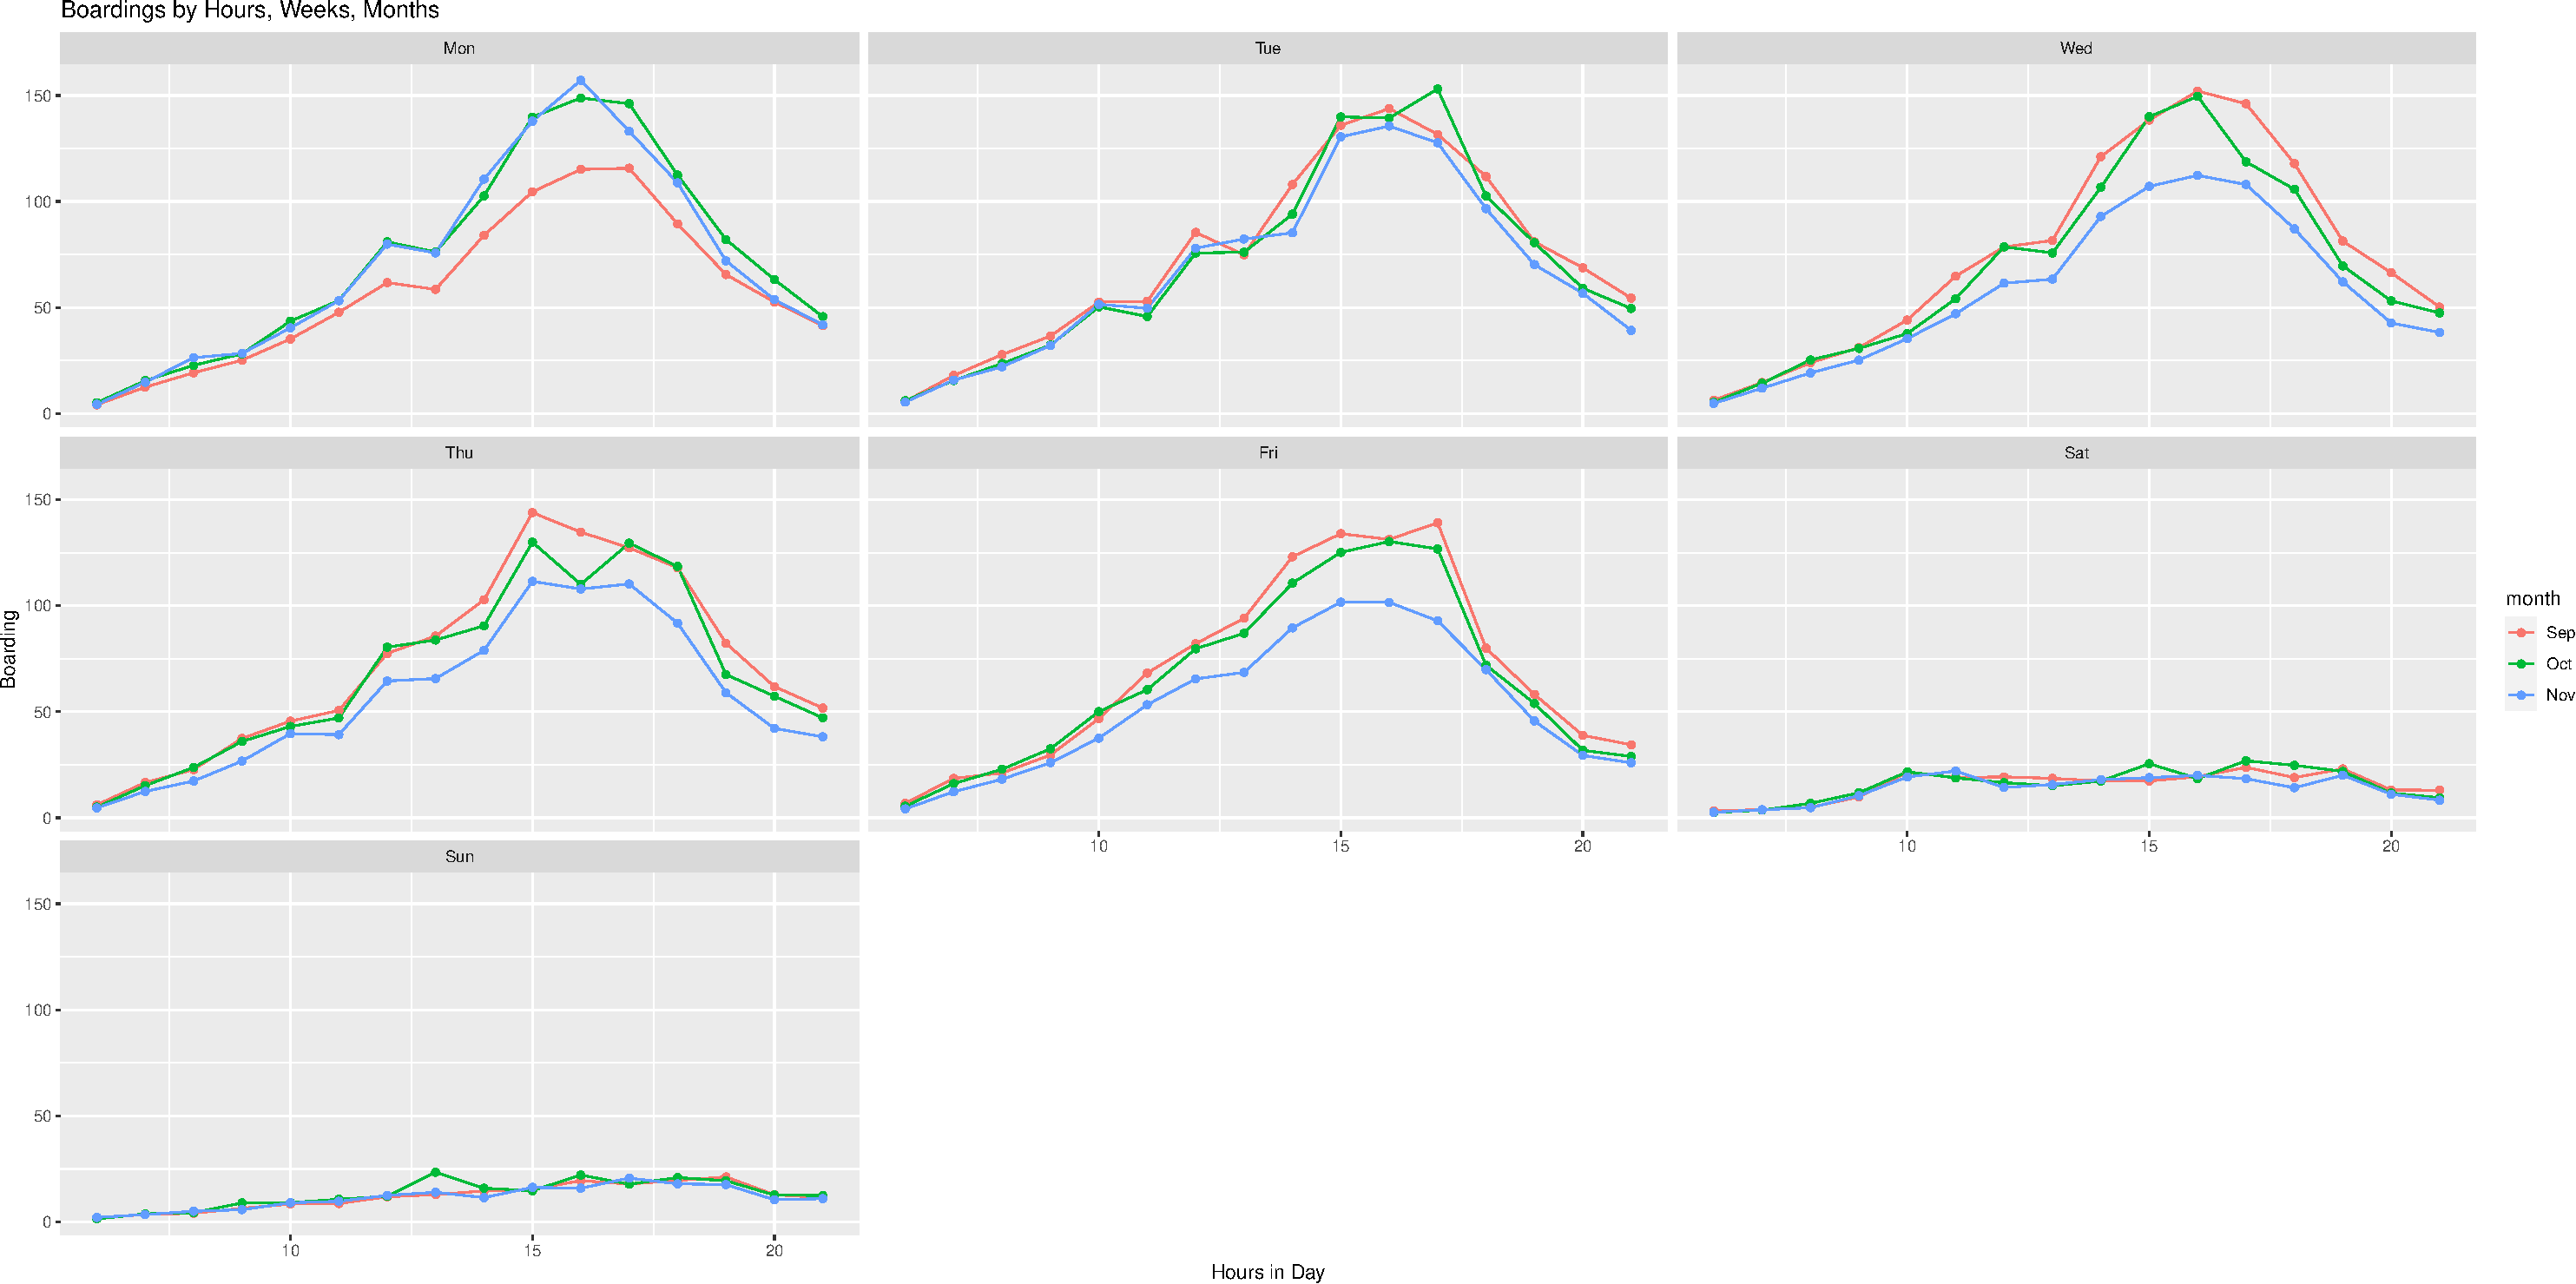
\includegraphics{_main_files/figure-latex/unnamed-chunk-28-1.pdf}

Caption: Above is the the combination of line plots above, each plot stands for a day in week. x-axis means the hours throughout a day from 6 a.m. to 9 p.m. The y-axis means the average boarding. We have 3 lines in each plot, representing 3 months from September to November. Orange line shows September, green line shows October, and blue line shows November.

Answer: From the combination of plots above, I found that the peak boarding from Monday to Friday are quite similar because these five days are workdays; students, teachers, and staffs are taking regular routines in these days. But, on weekend, the boarding curves become so flat because of no class and no work at school.

My reason for that the average boarding on Monday in September is lower than the other 2 months is September has a lot of new students coming. Most new students just know new friends and maybe hanging out with new friends on Sunday night. So, on Monday, they probably could not get up early enough to catch up a bus. That is why the average boarding on Monday is quite less than the other 2 months.

The average boarding on Weds/Thurs/Fri in November looks lower. I guess it is related to the Halloween Holiday. As we know, in Halloween, we have a short break and most people definitely do not come to school. Thus, undoubtedly, the average boarding should be lower.

\hypertarget{plot-2}{%
\subsubsection{Plot 2}\label{plot-2}}

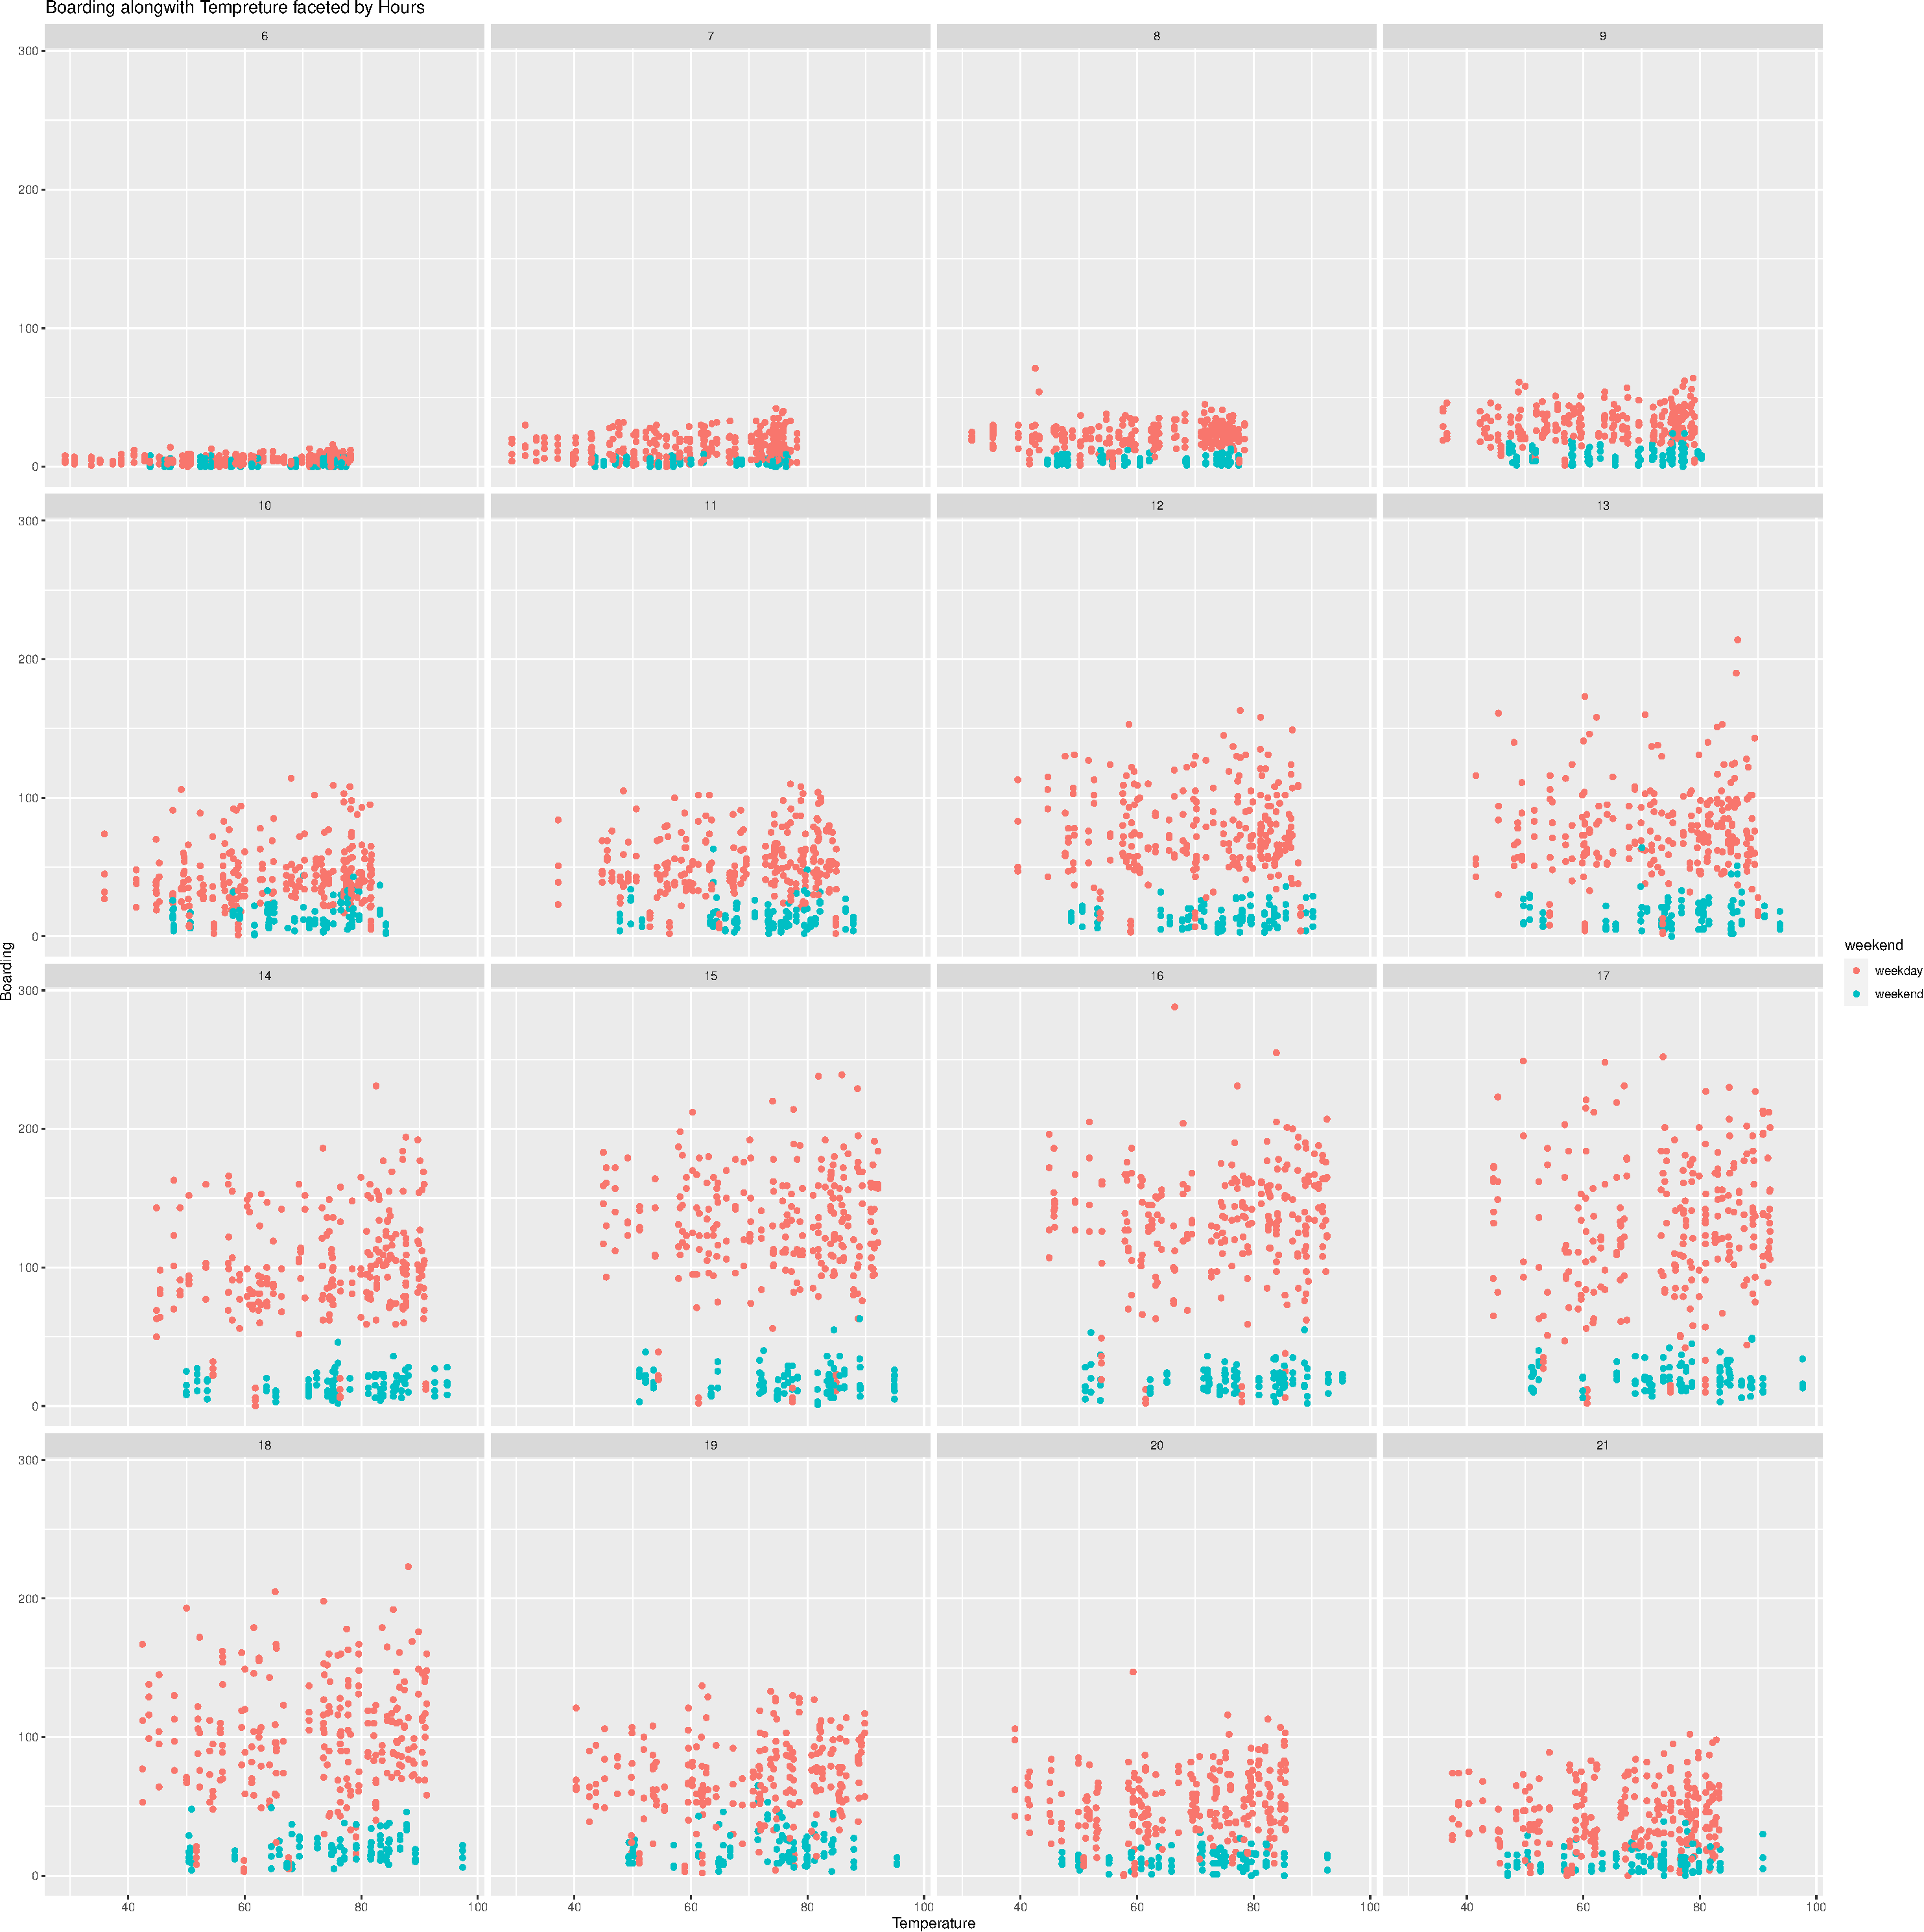
\includegraphics{_main_files/figure-latex/unnamed-chunk-29-1.pdf}

Caption: This combination of scatter plots shows the relationship between boarding number and temperature. The x-axis is temperature of each section and the y-axis is the boarding amount during each 15min section. Also each faceted plot stands for each hour from 6 a.m. to 9 p.m. e.g.~the first plot has a ``6'' above, which means 6 a.m. and the last plot has a 21 above which means 9 p.m.

Answer: Actually, I did not see any trend alongside with temperature. In each hour of days, the points distribution seems to be very chaotic and ruleless. Therefore, I dare to say temperature has no solid effect on the number of UT student boarding the bus.

\hypertarget{problem-2-wrangling-the-billboard-top-100}{%
\subsection{Problem 2 Wrangling the Billboard Top 100}\label{problem-2-wrangling-the-billboard-top-100}}

\hypertarget{part-a-3}{%
\subsubsection{Part A}\label{part-a-3}}

\begin{longtable}[]{@{}
  >{\centering\arraybackslash}p{(\columnwidth - 4\tabcolsep) * \real{0.4583}}
  >{\centering\arraybackslash}p{(\columnwidth - 4\tabcolsep) * \real{0.4306}}
  >{\centering\arraybackslash}p{(\columnwidth - 4\tabcolsep) * \real{0.1111}}@{}}
\toprule\noalign{}
\begin{minipage}[b]{\linewidth}\centering
performer
\end{minipage} & \begin{minipage}[b]{\linewidth}\centering
song
\end{minipage} & \begin{minipage}[b]{\linewidth}\centering
weeks
\end{minipage} \\
\midrule\noalign{}
\endhead
\bottomrule\noalign{}
\endlastfoot
Imagine Dragons & Radioactive & 87 \\
AWOLNATION & Sail & 79 \\
Jason Mraz & I'm Yours & 76 \\
The Weeknd & Blinding Lights & 76 \\
LeAnn Rimes & How Do I Live & 69 \\
LMFAO Featuring Lauren Bennett
\& GoonRock & Party Rock Anthem & 68 \\
OneRepublic & Counting Stars & 68 \\
Adele & Rolling In The Deep & 65 \\
Jewel & Foolish Games/You Were Meant
For Me & 65 \\
Carrie Underwood & Before He Cheats & 64 \\
\end{longtable}

Caption: This is the table for top 10 songs spending most weeks on the Billboard Top 100 from 1958 to 2021.

The first column shows the performer name of these songs, the second column lists the name of these songs, and the third colume stands for the total number of weeks for each song.

\hypertarget{part-b-3}{%
\subsubsection{Part B}\label{part-b-3}}

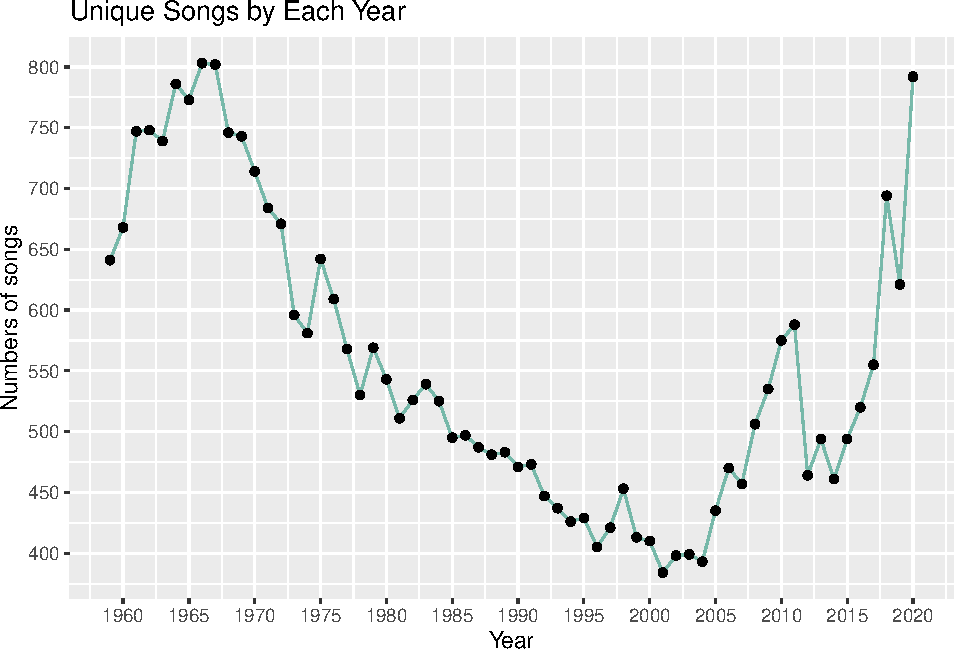
\includegraphics{_main_files/figure-latex/unnamed-chunk-32-1.pdf}

Caption: This is a line graph which shows the total amount of unique songs appearing in the Billboard Top 100 in each year from 1959 to 2020. x-axis represents the year and y-axis stands for the number of the songs.

Comment: I found that around the middle of 1960s, there was a peak which a lot of songs appearing in the Top List. I guess that one of potential reasons is that in these years, the hippie movement arose and gradually dominated the United States. Alongside with this movement, a lot of genres of music, like Rock\&Roll, R\&B, was becoming more and more popular. So during this time, songs were pretty diverse. Another rising trend seems to happen after 2010, maybe just because of globalization, songs from other cultures, such as K-pop, Latin, are becoming more and more public.

\hypertarget{part-3}{%
\subsubsection{Part 3}\label{part-3}}

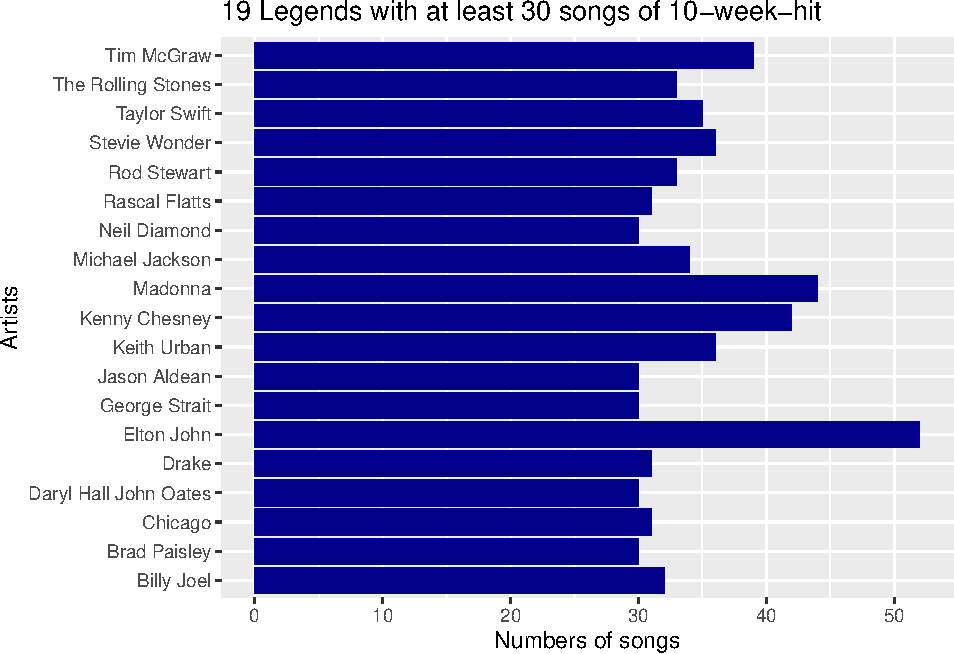
\includegraphics{_main_files/figure-latex/unnamed-chunk-33-1.pdf}

Caption: This is a bar plot showing 19 artists with equal or over 30 songs at least 10 weeks on the Billboard. The x-axis is the the number songs of each artist and the y-axis shows the name of each artist.

Sir Elton John has over 50 songs appearing more than 10 weeks in Billboard, which is a great achievement!

\hypertarget{problem-3-regression-practice}{%
\subsection{Problem 3 Regression Practice}\label{problem-3-regression-practice}}

Below is the intercept and estimated coefficient of age:

\begin{verbatim}
## (Intercept)         age 
## 147.8129158  -0.6198159
\end{verbatim}

Below shows the scatter plot of age(x-axis) and creatinine clearance rate(y-axis) with a reference line with the estimators above:

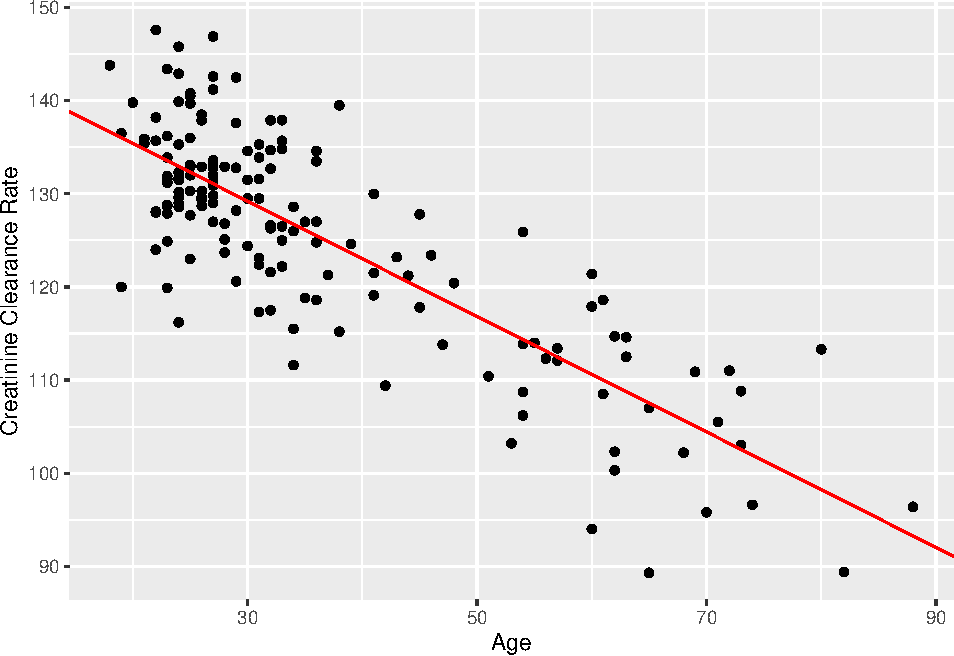
\includegraphics{_main_files/figure-latex/unnamed-chunk-36-1.pdf}

\hypertarget{part-a-4}{%
\subsubsection{Part A}\label{part-a-4}}

Let me put \emph{age = 55} i.e \emph{x = 55} into the equation \emph{y(creatinine) = 147.81 - 0.62x}. We can get:

\begin{verbatim}
## [1] 113.71
\end{verbatim}

So, we expect that a 55-year-old person has 113.71 ml/min creatinine clearance rate.

\hypertarget{part-b-4}{%
\subsubsection{Part B}\label{part-b-4}}

The coefficient of age told us that when we grow up 1 year, we expect to decrease 0.62 ml/min of creatinine clearance rate. i.e.~-0.62 ml/min per year.

\hypertarget{part-c-2}{%
\subsubsection{Part C}\label{part-c-2}}

Expected 40-year-old creatinine clearance rate:

\begin{verbatim}
## [1] 123.01
\end{verbatim}

Real rate: 135 ml/min

Expected 60-year-old creatinine clearance rate:

\begin{verbatim}
## [1] 110.61
\end{verbatim}

Real rate: 112 ml/min

So, we can know the difference between real creatinine clearance rate for the 40-year-old is \emph{135-123.01 = 11.99} and the difference between real creatinine clearance rate for the 60-year-old is \emph{112 - 110.61 = 1.39}. So from these two difference 11.99 is bigger than 1.39, we can say the 40-year old is healthier.

Let us look another comparison, the comparative rate which defines as \emph{difference/expected value}:

For the 40:

\begin{verbatim}
## [1] 0.097
\end{verbatim}

For the 60:

\begin{verbatim}
## [1] 0.013
\end{verbatim}

So, the rate of the 40 is almost 9 times of the rate of the 60, which means the 40 is comparatively healthier than the expected value for 40.

In conclusion, the 40-year-old is healthier than the 60-year-old in terms of creatinine clearance rate.

\hypertarget{problem-4-probability-practice}{%
\subsection{Problem 4 Probability Practice}\label{problem-4-probability-practice}}

\hypertarget{part-a-5}{%
\subsubsection{Part A}\label{part-a-5}}

Let event A be buying 3 cars and none of them is lemon.

So, \textasciitilde A should be buying 3 cars and at least one of them is lemon.

\emph{P(\textasciitilde A) = 1 - P(A) =}

\begin{verbatim}
## [1] 0.719
\end{verbatim}

The probability of getting at least one lemon should be 72\%.

\hypertarget{part-b-5}{%
\subsubsection{Part B}\label{part-b-5}}

Since each time of throwing a dice is independent, we can treat throwing a dice twice as independent events.

For the probability of getting the sum of 2 number is odd, we have 2 scenarios: First, first time is a even and second time is a odd; the other is converse. So the probability of this event should be \emph{P(odd) * P(even) + P(even) * P(odd)}, which is

\begin{verbatim}
## [1] 0.5
\end{verbatim}

For the probability of the sum of 2 number is less than 7, we can go through case by case. If we get 1 at first time, we can get 1,2,3,4,5 at the second time, the probability of it should be 1/6 * 5/6 = 5/36. If we get 2 at first time, we can get 1,2,3,4 at the second time, the P of it should be 1/6 * 4/6 = 4/36. If getting 3 at the first time, the P should be 1/6 * 3/6 = 3/36. If 4, then 1/6 * 2/6 = 2/36. If 5, then 1/6 * 1/6 = 1/36. If 6, no chance to get less than 7, so the P is 0. Then we add up these probabilities, we can get

\begin{verbatim}
## [1] 0.417
\end{verbatim}

So the chance to get the sum of 2 numbers less than 7 is about 42\%

In this cas, we can go through case by case again. If we get 1 at first time, we can get 2,4 at the second time, 2 cases here. If we get 2 at first time, we can get 1,3 at the second time, 2 cases hear. If getting 3 at the first time, we can get 2 at second time, then 1 case. If 4, then get 1 at second time, still 1 case. If 5, then 0. Then we add up these case, we can get 6 case.

The total case is 6 * 6=36, and the chance of getting odd number is 0.5, so the odd case is 0.5 * 36 = 18.

Thus, the P(\textless7\textbar the number is odd) = 6/18 = 1/3

If they are independent, then P(A\textbar B) = P(A), but here, P(\textless7) = 0.42 and P(\textless7\textbar odd) = 0.33. Therefore, they are not independent apparently.

\hypertarget{part-c-3}{%
\subsubsection{Part C}\label{part-c-3}}

Information we already have:

P(RC) = 0.3

P(TC) = 0.7

P(yes\textbar RC) = 0.5

P(no\textbar RC) = 0.5

P(yes) = 0.65

P(no) = 0.35

What we need to get: P(yes\textbar TC)

P(yes) = P(RC) * P(yes\textbar RC) + P(TC) * P(yes\textbar TC), which is 0.65 = 0.3 * 0.5 + 0.7 * x

Solve the equation, we get

\begin{verbatim}
## [1] 0.714
\end{verbatim}

Thus, there are 71\% Truthful visitors saying yes in the survey.

\hypertarget{part-d-1}{%
\subsubsection{Part D}\label{part-d-1}}

Given information:

P(positive\textbar disease) = 0.993

P(negative\textbar non-disease) = 0.999

P(disease) = 0.000025

P(non-disease) = 1 - 0.000025 = 0.999975

What we need to get: P(disease\textbar positive) by Bayes Rule

P(positive\textbar non-disease) = 1 - P(negative\textbar non-disease) = 0.0001

P(positive) = P(positive\textbar disease) * P(disease) + P(positive\textbar non-disease) * P(non-disease) =

\begin{verbatim}
## [1] 0.0001248225
\end{verbatim}

P(disease\textbar positive) = P(positive\textbar disease) * P(disease) / P(positive) =

\begin{verbatim}
## [1] 0.1988784
\end{verbatim}

So, there is 19.9\% chance someone have the disease when testing positive.

\hypertarget{part-e}{%
\subsubsection{Part E}\label{part-e}}

Given Information:

P(R/A) = 0.99

P(R/\textasciitilde A) = 0.10

P(A) = 0.05

P(\textasciitilde A) = 0.95

Need to show: P(A/R)

P(R) = P(A) * P(R/A) + P(\textasciitilde A) * P(R/\textasciitilde A) =

\begin{verbatim}
## [1] 0.1445
\end{verbatim}

P(A/R) = P(R/A) * P(A) / P(R) =

\begin{verbatim}
## [1] 0.3425606
\end{verbatim}

So, the probability of that an aircraft is present given it is registered should be around 34.26\%

\hypertarget{problem-5-modeling-soccer-games-with-th-poisson-distribution}{%
\subsection{Problem 5 Modeling soccer games with th Poisson distribution}\label{problem-5-modeling-soccer-games-with-th-poisson-distribution}}

In order to answer the question what are the estimated probabilities of win/lose/draw results between 2 teams, we need to use the Probability Mass Function of Poisson Distribution to calculate the probabilities of all possible goals for both teams.

The PMF of Poisson distribution takes the following form:

\[
P(X=x)=(λ^x/x!)e^−λ
\]

λ means the expected goals for each team and event X means how many goals scored in a game.

Approach: First, I need to make an assumption that the goals scored by each team is an independent event. So, when a probability of a game score(like 2-1) should be the probability of first team scoring 2 goals times the probability of second team scoring 1 goal.

Find the λ (expected goal by a team) by the formula:

\textbf{The team's attach power * The rival's defense weakness * Home/away boost}, in which:

Attach power = The total goals for a team in a season/the average goals of all teams in a season

Defense weakness = The total goals lost by a team in a season/the average goals lost of all teams in a season

Home boost = the average goals for all home teams in a match

Away boost = the average goals for all away teams in a match

After we get λ, we need to use PMF of Poisson to calculate a probabilty of an outcome. For example:

Set team A's λ is 1.5 and team B's λ is 1.7, then the goal for A is Xa and the goal for B is Xb.

Since Xa and Xb are independent, we have

\[
P(Xa=2,Xb=1) = (1.5^2/2!)e^−1.5 * (1.7^1/1!)e^−1.7
\]

With just a little bit more work, we can use calculate the probability of all possible outcomes up to a rip-roaring (but very unlikely) 7-7 draw by `tibble', `expand', `mutate' functions in R.

Then, we have a table for all probabilities of games from 0-0 to 7-7 (64 outcomes). Then by `filter' function, we can calculate the probability of each scenario(win/lose/draw).

\textbf{Next, Let me calculate the home/away boost, and seasonal average goals for further use}

The average number of goals scored i.e.~conceded by teams is (all the goals/20 teams):

\begin{verbatim}
## [1] 53.6
\end{verbatim}

The home boost is

\begin{verbatim}
## [1] 1.57
\end{verbatim}

The away boost is

\begin{verbatim}
## [1] 1.25
\end{verbatim}

\hypertarget{question-1}{%
\subsubsection{Question 1}\label{question-1}}

Liverpool(home) vs Tottenhan(away)

The Attack Strength for Liverpool(home) sould be:

\begin{verbatim}
## [1] 1.66
\end{verbatim}

The Defense Weakness for Liverpool(home) should be:

\begin{verbatim}
## [1] 0.41
\end{verbatim}

The Attack Strength for Tottenhan(away) should be:

\begin{verbatim}
## [1] 1.25
\end{verbatim}

The Defense Weakness for Tottenhan(away) should be:

\begin{verbatim}
## [1] 0.73
\end{verbatim}

The λ for Liverpool(home) should be:

\begin{verbatim}
## [1] 1.89
\end{verbatim}

The λ for Tottenhan(away) should be:

\begin{verbatim}
## [1] 0.64
\end{verbatim}

Now, we have the λs for both Liverpool and Tottenhan.

Now, show head 5 rows in a probabilities table for all possible game scores up to 6-6:

Liverpool

Tottenhan

prob

1

0

0

0.079

2

0

1

0.051

3

0

2

0.016

4

0

3

0.003

5

0

4

0.001

Then visualize it by heatmap:

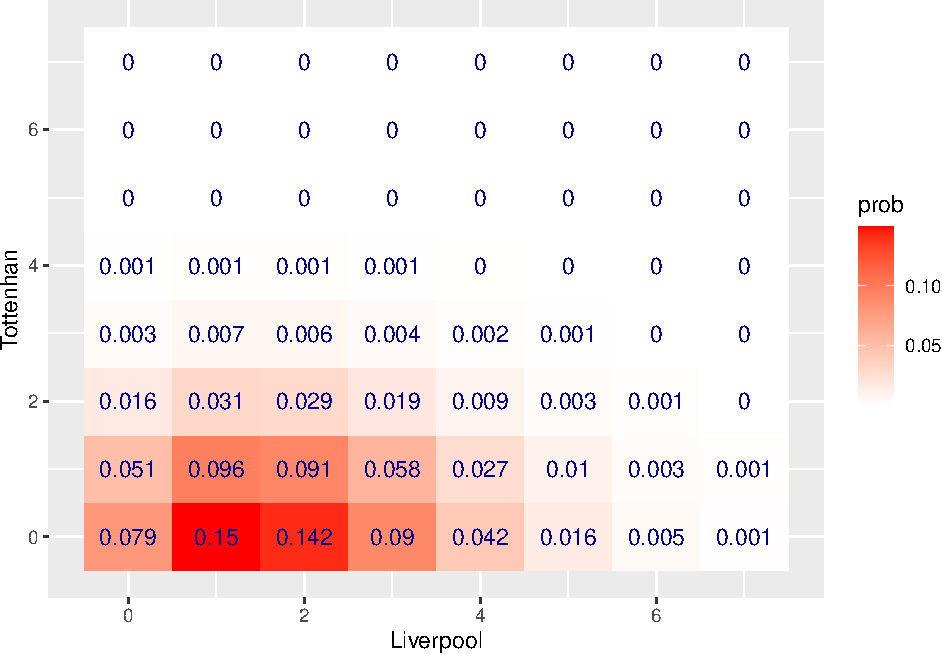
\includegraphics{_main_files/figure-latex/unnamed-chunk-61-1.pdf}

Then calculate the probabilities of 3 scenarios:

Liverpool win:

\begin{verbatim}
## # A tibble: 1 x 1
##   `sum(prob)`
##         <dbl>
## 1       0.672
\end{verbatim}

Tottenhan win:

\begin{verbatim}
## # A tibble: 1 x 1
##   `sum(prob)`
##         <dbl>
## 1       0.118
\end{verbatim}

Draw:

\begin{verbatim}
## # A tibble: 1 x 1
##   `sum(prob)`
##         <dbl>
## 1       0.209
\end{verbatim}

In conclusion, the chance of Liverpool winning is around 67.2\%, the chance of Tottenhan winning is 11.8\%, and the chance of draw is 20.9\%

\hypertarget{question-2}{%
\subsubsection{Question 2}\label{question-2}}

Manchester City(home) vs Arsenal(away)

The Attack Strength for Manchester City(home) sould be:

\begin{verbatim}
## [1] 1.77
\end{verbatim}

The Defense Weakness for Manchester City(home) should be:

\begin{verbatim}
## [1] 0.43
\end{verbatim}

The Attack Strength for Arsenal(away) should be:

\begin{verbatim}
## [1] 1.36
\end{verbatim}

The Defense Weakness for Arsenal(away) should be:

\begin{verbatim}
## [1] 0.95
\end{verbatim}

The λ for Manchester City(home) should be:

\begin{verbatim}
## [1] 2.65
\end{verbatim}

The λ for Arsenal(away) should be:

\begin{verbatim}
## [1] 0.73
\end{verbatim}

Now, we have the λs for both Liverpool and Tottenhan.

Now, show head 5 rows in a probabilities table for all possible game scores up to 7-7:

ManchesterCity

Arsenal

prob

1

0

0

0.034

2

0

1

0.025

3

0

2

0.009

4

0

3

0.002

5

0

4

0.000

Then visualize it by heatmap:

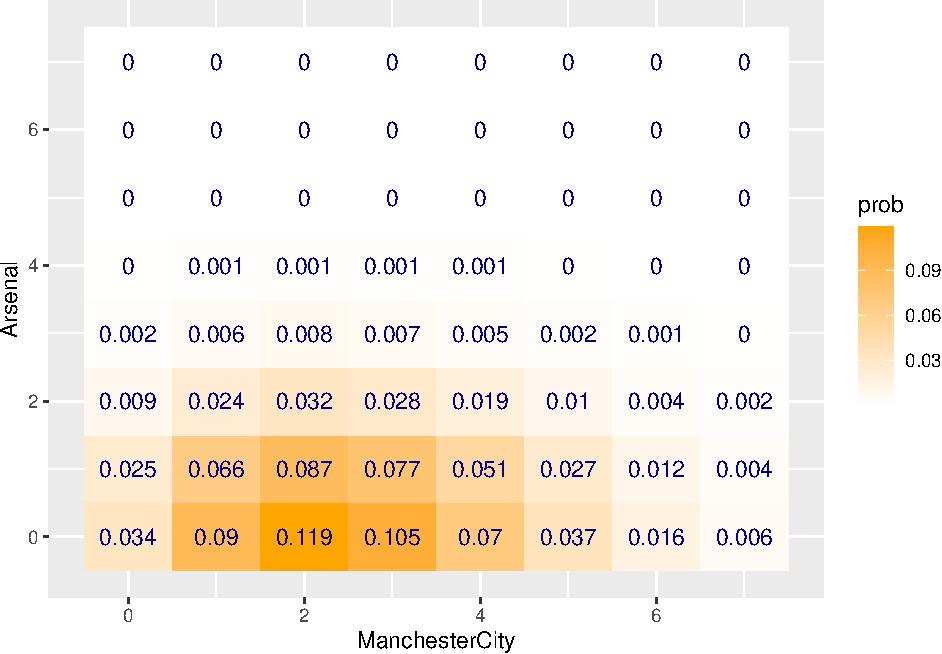
\includegraphics{_main_files/figure-latex/unnamed-chunk-72-1.pdf}

Then calculate the probabilities of 3 scenarios:

ManchesterCity win:

\begin{verbatim}
## # A tibble: 1 x 1
##   `sum(prob)`
##         <dbl>
## 1       0.775
\end{verbatim}

Arsenal win:

\begin{verbatim}
## # A tibble: 1 x 1
##   `sum(prob)`
##         <dbl>
## 1      0.0793
\end{verbatim}

Draw:

\begin{verbatim}
## # A tibble: 1 x 1
##   `sum(prob)`
##         <dbl>
## 1       0.140
\end{verbatim}

In conclusion, the chance of ManchesterCity winning is around 77.5\%, the chance of Arsenal winning is 7.9\%, and the chance of draw is 14\%

\hypertarget{homework-3}{%
\section{Homework 3}\label{homework-3}}

\hypertarget{problem-1-cdfs-and-pdfs}{%
\subsection{Problem 1 CDFs and PDFs}\label{problem-1-cdfs-and-pdfs}}

\hypertarget{part-a-6}{%
\subsubsection{Part A}\label{part-a-6}}

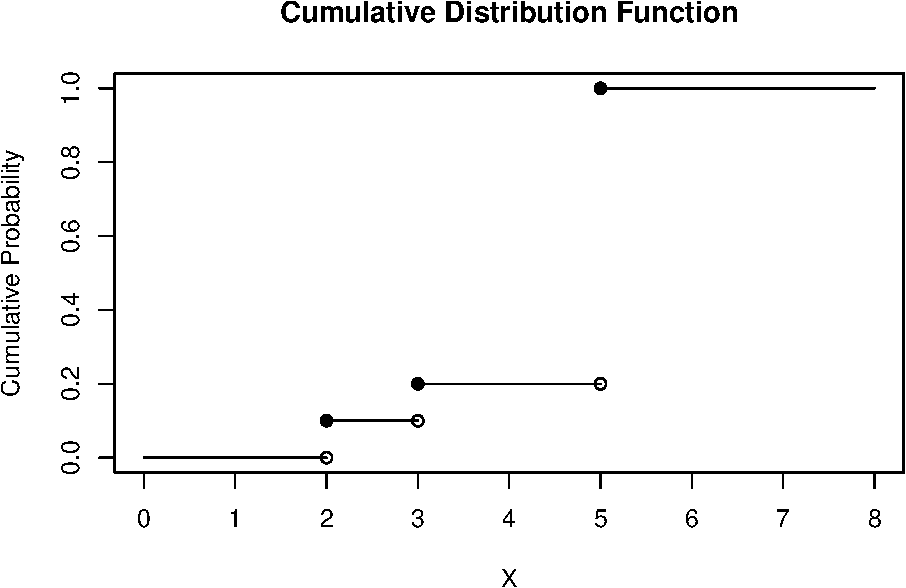
\includegraphics{_main_files/figure-latex/unnamed-chunk-77-1.pdf}

The CDF's plot shows above. X is the event, and Y-axis shows the cumulative probability.

We can conclude that:

\[
P(2< X ≤ 4.5) = P(X = 3) = 0.1
\]

\[
P(2 ≤ X < 4.5) = P(X = {2,3}) = 0.1 + 0.1 = 0.2.
\]

\hypertarget{part-b-6}{%
\subsubsection{Part B}\label{part-b-6}}

\hypertarget{i}{%
\paragraph{(i)}\label{i}}

\[
P(X^2 ≤ 0.25) = P (X ≤ \sqrt{0.25}) = P(X≤ 0.5)
\]

Since it follows a uniform distribution, then by the formula

\[
P(X≤ 0.5) = \frac{0.5-0}{1-0} = 0.5
\]

\hypertarget{ii}{%
\paragraph{(ii)}\label{ii}}

We have to make clear that 0 \textless{} a \textless{} 1, otherwise it will fail to get a probability.

\[
P(X^2 ≤ a) = P (X ≤ \sqrt{a}) = \frac{\sqrt{a}-0}{1-0} = \sqrt{a}
\]

\hypertarget{iii}{%
\paragraph{(iii)}\label{iii}}

From part (ii), we know that

\[
P(Y≤ y) = P(X^2 ≤ y) = P (X ≤ \sqrt{y}) = \frac{\sqrt{y}-0}{1-0} = \sqrt{y}
\]

So the CDF of Y is:

\[
F(y) = \sqrt{y}
\]

And then take first-order derivatives to PDF:

\[
f_y(y) = \frac{d(\sqrt{y})}{dy} = \frac{1}{2(\sqrt{y})}
\]

\hypertarget{iiii}{%
\paragraph{(iiii)}\label{iiii}}

Compute E(Y):

\[
E(Y) = \int_{0}^{1} yf(y)dy = \int_{0}^{1} \frac{y}{2(\sqrt{y})}dy =\int_{0}^{1}  \frac{\sqrt{y}}{2}dy = \frac{1}{3}*(1)^\frac{3}{2} - 0 = \frac{1}{3}
\]

In order to compute var(Y), we need to calculate E(Y\^{}2) first.

Compute E(Y\^{}2):

\[
E(Y^2) = \int_{0}^{1} y^2f(y)dy = \int_{0}^{1} \frac{y^2}{2(\sqrt{y})}dy =\int_{0}^{1}  \frac{\sqrt{y^3}}{2}dy = \frac{1}{5}*(1)^\frac{5}{2} - 0 = \frac{1}{5}
\]

Thus, the var(Y) = E(Y\^{}2) - E(Y)\^{}2 as follow:

\[
var(Y) = E(Y^2)- E(Y)^2 = \frac{1}{5} - (\frac{1}{3})^2 = \frac{4}{45}
\]

\hypertarget{problem-2-practice-with-expected-value}{%
\subsection{Problem 2 Practice with Expected Value}\label{problem-2-practice-with-expected-value}}

\hypertarget{part-a-7}{%
\subsubsection{Part A}\label{part-a-7}}

We are trying to get E(X):

\[
E(X) = E(Z_1^2+Z_2^2...+Z_d^2) = E(Z_1^2)+E(Z_2^2)+...+E(Z_d^2)
\] Since Z\_1 to Z\_d are all follows the same distribution, we have:

\[
E(Z_1^2) = E(Z_2^2) = ... = E(Z_d^2)
\]

Thus, as long as we get E(Z\_i\^{}2), we are done. So the E(Z\_i\^{}2):

\[
E(Z_i^2) = Var(Z_i) + E(Z_i)^2 = 1 + 0^2 = 1
\]

The we can get E(X):

\[
E(X) =E(Z_1^2)+E(Z_2^2)+...+E(Z_d^2) = \sum_{i = 1}^{d} 1 = d
\]

\hypertarget{part-b-7}{%
\subsubsection{Part B}\label{part-b-7}}

I do not agree with that, because average velocity does not take into account the time spent at different velocities during the entire journey.

Therefore, if we want to figure out the average time, we should calculate the time for walking and biking separately, and then take weighted average of them.

Thus, the time for walking should be:

\[
T(walking) = Distance/Velocity(walking) =2(miles)/5(miles/hour) = 0.4 hour
\]

And the time for biking should be:

\[
T(biking) = Distance/Velocity(biking) =2(miles)/10(miles/hour) = 0.2 hour
\]

And the add in the probabilities of two situations, we have:

\[
T = w(walking)*T(walking) + w(biking)*T(biking) \\= 0.4*0.4 + 0.6*0.2 = 0.16 +0.12 = 0.28 hour = 16.8 minutes
\]

Thus, Markov takes average 0.28 hour, or 16.8 minutes, to get to the class.

\hypertarget{problem-3-inverse-cdf}{%
\subsection{Problem 3 Inverse CDF}\label{problem-3-inverse-cdf}}

We can calculate the P(X\textless x) first:

\[
P(X≤x) = P(F^{-1}(U)≤x) = P(F(F^{-1}(U))≤F(x)) = P(U≤F(x)) = F(x)
\]
Then once we get the CDF, we can get the PDF of it.

\[
f(x) = F'(x) 
\]

Let's look at the detailed case here (0≤u≤1):

\[
F(u) = P(U≤u) = \frac {u-0}{1-0} = u
\]

The plot as followed:

\begin{verbatim}
## Warning in title(...): conversion failure on 'U≤u' in 'mbcsToSbcs': dot
## substituted for <e2>
\end{verbatim}

\begin{verbatim}
## Warning in title(...): conversion failure on 'U≤u' in 'mbcsToSbcs': dot
## substituted for <89>
\end{verbatim}

\begin{verbatim}
## Warning in title(...): conversion failure on 'U≤u' in 'mbcsToSbcs': dot
## substituted for <a4>
\end{verbatim}

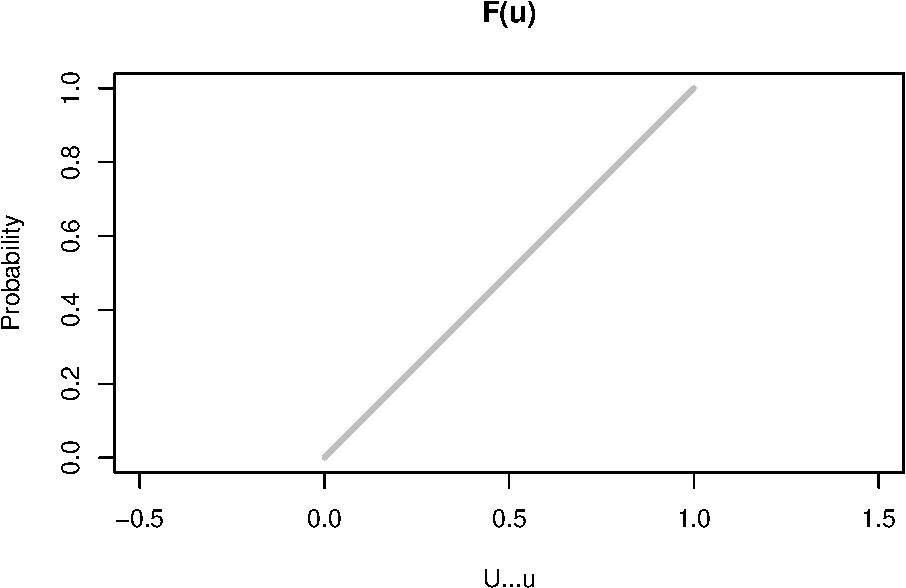
\includegraphics{_main_files/figure-latex/unnamed-chunk-78-1.pdf}

Since X = F\^{}-1(U), we can see from the picture X and U are identical and all a uniform distribution on {[}0,1{]}. Thus, we can conclude that the pdf of f(x) equals to of f(u) as followed (0≤x≤1):

\[
f(x) = \frac {1}{1-0} = 1 
\]

The plot shows as followed:

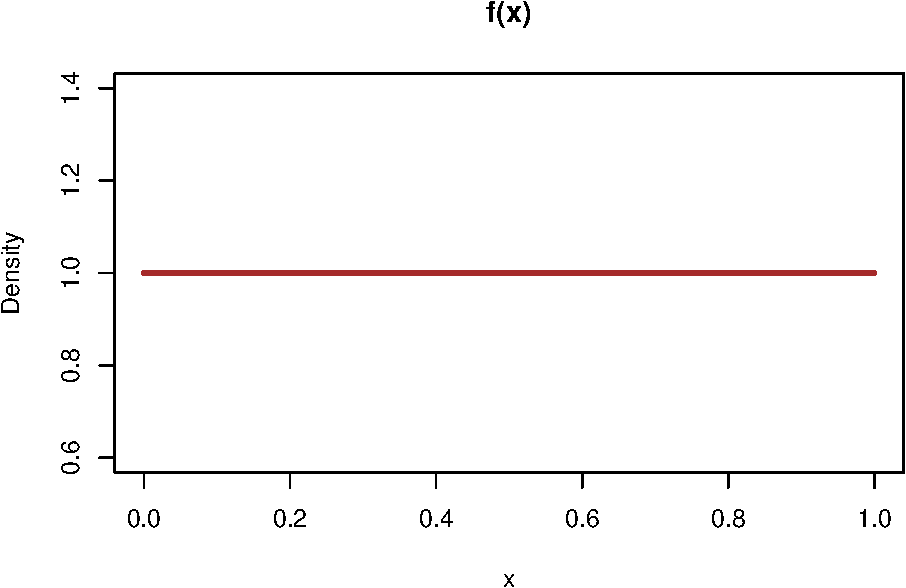
\includegraphics{_main_files/figure-latex/unnamed-chunk-79-1.pdf}

\hypertarget{problem-4-simulation}{%
\subsection{Problem 4 Simulation}\label{problem-4-simulation}}

\hypertarget{part-a-8}{%
\subsubsection{Part A}\label{part-a-8}}

The expected value for pn shows below:

\[
E(\hat{p_N}) = E(\frac{X_N}{N}) = \frac{E(X_N)}{N} = \frac{NP}{N} = P
\]

The standard deviation for pn shows below:

\[
sd(\hat{p_N}) = \sqrt {(var(\hat{p_N}))} = \sqrt {var(\frac{X_N}{N})}_ = \sqrt {\frac{var(X_N)}{N^2}} = \sqrt \frac{NP(1-P)}{N^2} = \sqrt{\frac {P-P^2}{N}}
\]

\hypertarget{part-b-8}{%
\subsubsection{Part B}\label{part-b-8}}

If we put N=5, P=0.5 in formula E(P\_N) and sd(P\_N), we can get:

Probability for N=5:

\begin{verbatim}
## [1] 0.5
\end{verbatim}

Standard deviation for N=5:

\begin{verbatim}
## [1] 0.2236
\end{verbatim}

Then we use randomly simulate 1000 times, we can get Monte Carlo Mean:

\begin{verbatim}
## [1] 0.5146
\end{verbatim}

Monte Carlo Standard Deviation:

\begin{verbatim}
## [1] 0.2191
\end{verbatim}

From the results above, we can find Monte Carlo Mean is very close to theoretical mean, and of cause, Monte Carlo standard deviation basically agrees with the theoretical standard deviation.

Repeat the same process for p10, p25, p50, p100, and make the plot as required below:

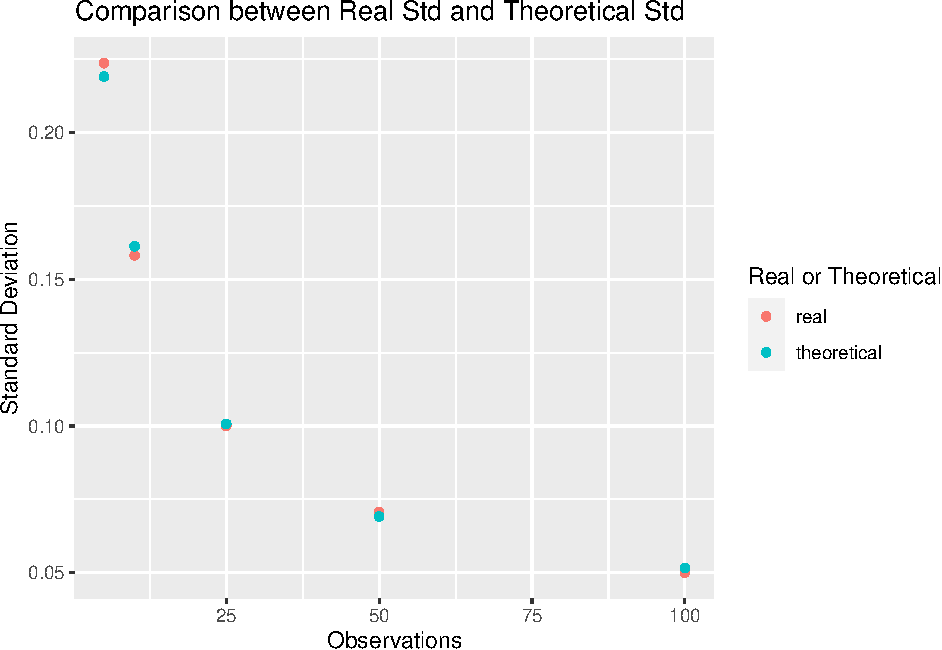
\includegraphics{_main_files/figure-latex/unnamed-chunk-84-1.pdf}

Caption: X-axis stands for the observation times in an experiment, noted as N; Y-axis represents the value of standard deviation. Besides, orange points mean the real value from experiments, and blue points are the theoretical value calculated be the formula in Part (A).

Comments: From the plot above, we can see that, as the observations(N) of experiment increase more and more, the standard deviation become less and less, which matches the standard deviation formula in part (A).

In addition to that, I can find that, as the observations(N) of each experiment increase, the real standard deviations are more close to the theoretical standard deviations.It complies large number theorem.

\hypertarget{problem-5-more-pdfcdf-practice}{%
\subsection{Problem 5 More PDF/CDF Practice}\label{problem-5-more-pdfcdf-practice}}

The CDF of X\_i(i=1,2,\ldots,N) as given:

\[
F_{X_i}(x) = P(X_i≤x) = \int_{0}^{x} \lambda e^{-\lambda t}dt = 1- e^{-\lambda x}
\]

Since max\{X\_i(i=1,2,\ldots,N)\}) \textless{} y is equivalent to X\_i \textless{} y for any i, then we have:

\[
F_{Y_N}(y) = P(Y_N < y) \\= P(max(X_1,X_2...X_N)<y) \\= P(X_1<y,X_2<y,X_3<y...X_N<y)
\]

And then because X itself is independent, then we have:

\[
P(X_1<y,X_2<y,X_3<y...X_N<y) \\= P(X_1<y) *P(X_2<y) *...*P(X_N<y) \\= F_{X_1}(y)*F_{X_2}(y)*...*F_{X_N}(y) \\= (1- e^{-\lambda y})^N
\]
Then, differentiate the CDF of Y\_N, we can get the PDF of Y\_N:

\[
f_{Y_N} = \frac {dF_{Y_N}(y)}{dy} = \frac {d}{dy}(1-e^{\lambda y})^N = N(1-e^{\lambda y})^{N-1}*(-e^{-\lambda y})*-\lambda = N\lambda e^{-\lambda y}(1-e^{-\lambda y})^{N-1}
\]

  \bibliography{book.bib,packages.bib}

\end{document}
